\section{2048のミニゲームの完全解析}
\label{chap:solving}
\ref{chap:rl}章で述べた強化学習は環境~(ゲーム)~と何度もやり取りすることで, 最適な方策を学習するための手法である.
一方で小さなゲームであれば, 力ずくの計算によってゲームを完全に解くこともできる.
本節では2048を解析的なアプローチによって解くことについて述べる.
なお本節の内容は文献~\cite{3x3_2048}および文献~\cite{4x3_2048}を元に執筆された.

\subsection{2048の完全解析とは}
\label{sec:solving}
2048は$1$人用のゲームであるため, 勝敗のようなプレイヤの明確な目標は存在しない.
そのためプレイヤが何を目標とするかによって, プレイヤの最善手の定義は変化する.
また\ref{sec:rule}節で述べたようにゲームはランダム性を伴うため, 同じ状態から毎回同じ手を選んでも結果は確率的に変動する.

そこで本稿ではある状態$s$における最善手を「$s$から獲得できる得点の合計の期待値が最も高くなるような手」と定義する.
これは~\ref{chap:rl}節で述べた強化学習の最適状態価値と等価なものである.
よって状態$s$から最善手を選び続けて獲得できる得点の合計の期待値を状態$s$の最適価値と呼び, $v_*(s)$で表すことにする.

このとき$v_*(s)$は式~\ref{eq:value}のように再帰的な形式で書くことができる.
\begin{align}
    v_*(s) =
    \begin{cases}
        0 & (s \text{が終了状態}) \\
        \max_a \left(r(s,a) + \mathbb{E}_{s_\text{next} \in \mathcal{T}(s,a)} v_*(s_\text{next}) \right) & (\text{otherwise})
    \end{cases}
    \label{eq:value}
\end{align}
ただし$r(s,a)$は状態$s$から行動$a$をとって獲得する得点, $s_\text{next} \in \mathcal{T}(s,a)$は状態$s$から行動$a$をとって遷移しうる次の状態の集合を表す~(図~\ref{fig:state_afterstate}を参照).
式~\ref{eq:value}の$r(s,a) + \mathbb{E}_{s_\text{next} \in \mathcal{T}(s,a)} v_*(s_\text{next})$は, 強化学習における最適行動価値$q_*(s,a)$に対応する.
また$\mathbb{E}_{s_\text{next} \in \mathcal{T}(s,a)} v_*(s_\text{next})$は, $s$から$a$をとって遷移するafterstate $s'$の価値といえる.

\begin{figure}[t]
    \centering
    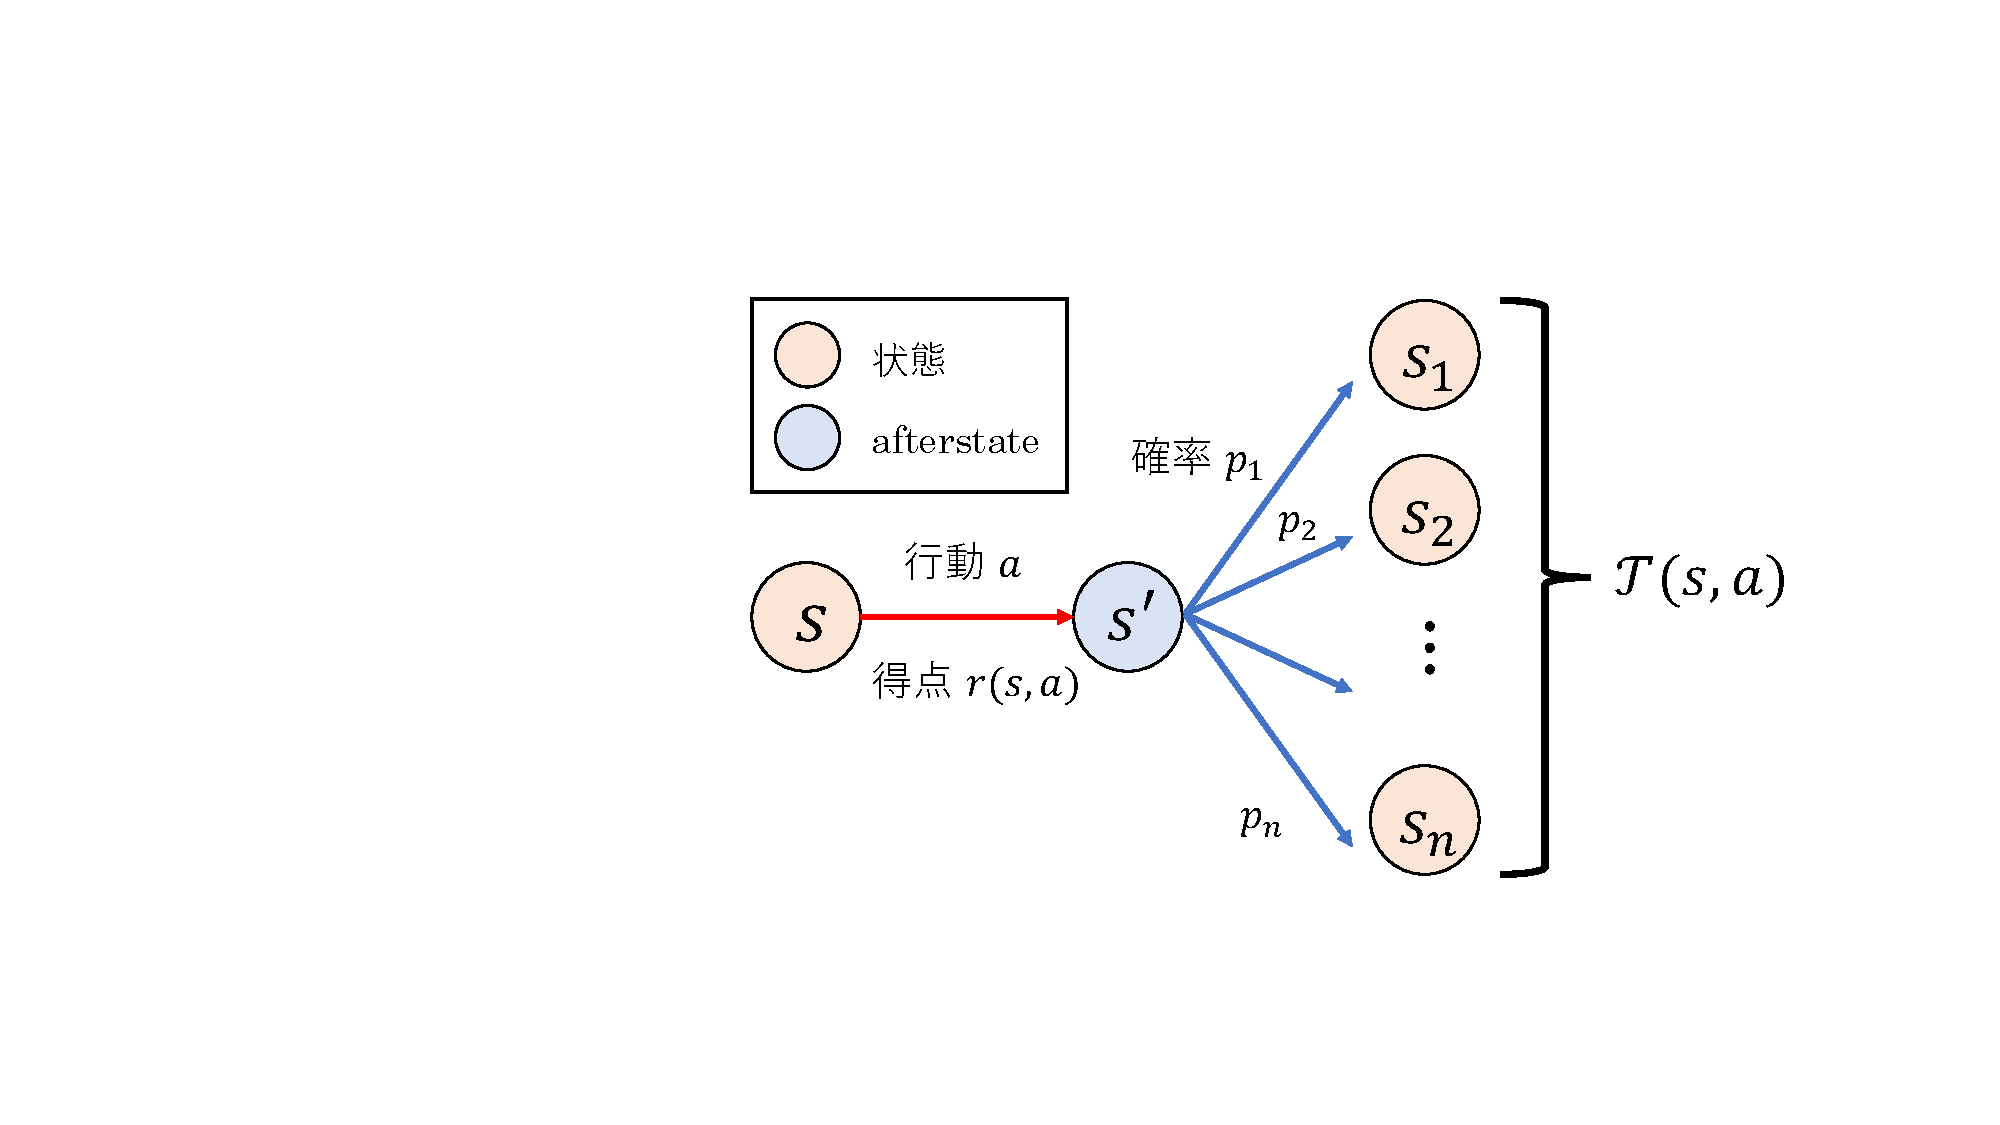
\includegraphics[width=0.6\linewidth{}]{figures/value_function_.pdf}
    \caption{式~\ref{eq:value}の補足図}
    \label{fig:state_afterstate}
\end{figure}

ゲームに現れうるすべての状態の最適価値を計算すれば, 任意の状態において最善手を選ぶことができる.
本稿ではこれを2048の完全解析ということにする.

完全解析をすることで, ゲームの任意の状態の最適価値・最善手を明かし, 最善手を選び続けるプレイヤの戦略を解析することができる.
さらに2048を対象とした強化学習手法の良し悪しを, 定量的な指標によって評価することができると考えられる.
一方で2048を完全解析することは, そのゲーム木の大きさによる計算コストの観点から現状難しいと考えられる.
そこで本研究では本来$4\times4$盤面上で行われる2048のミニゲームとして, 盤面サイズを縮小した2048を完全解析することを提案する.
\begin{figure} 
\centering
\begin{subfigure}[T]{0.2\columnwidth}
    \centering
    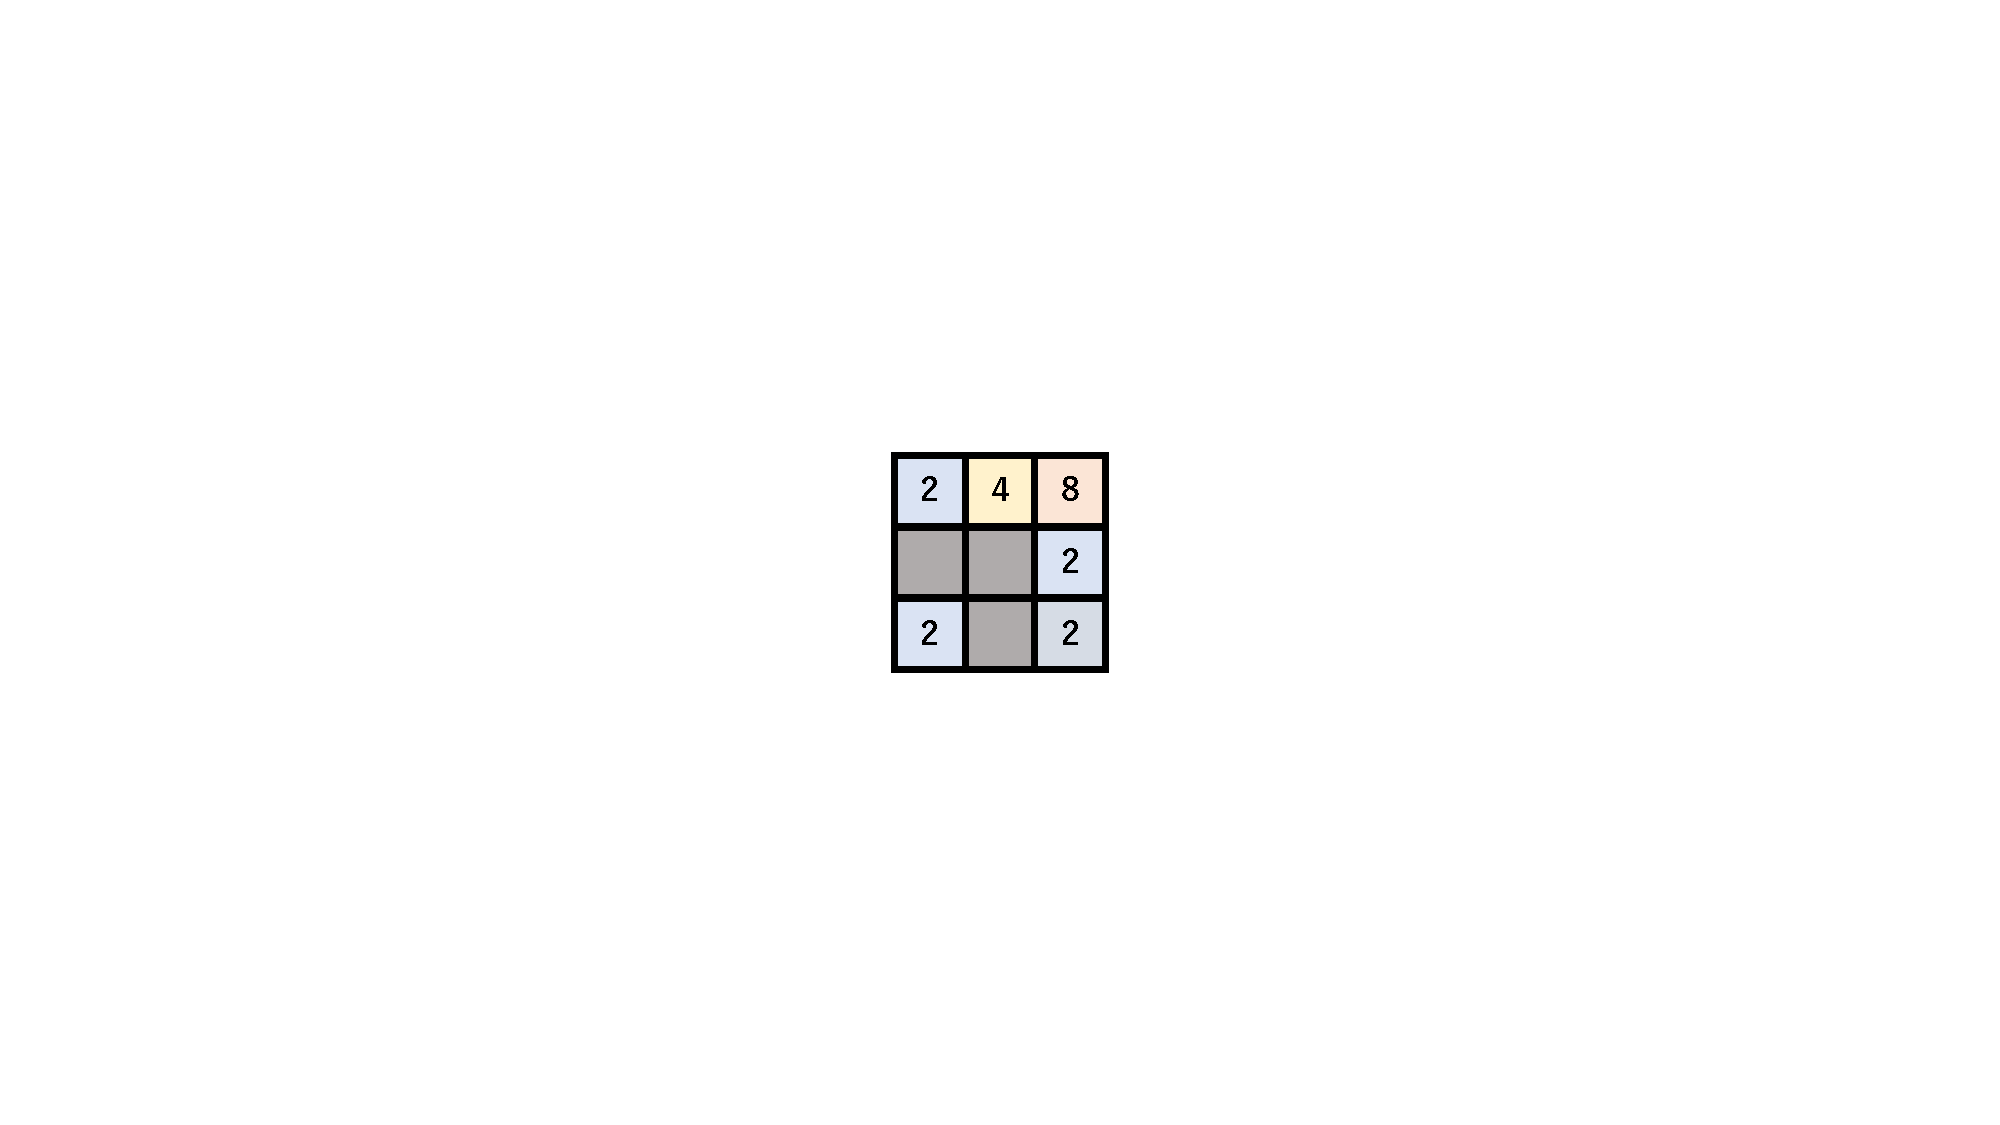
\includegraphics[width=\columnwidth]{figures/mini2048.pdf}
    \caption{$3\times3$盤面の2048}
    \label{fig:mini2048}
\end{subfigure}
\hspace{1cm}
\begin{subfigure}[T]{0.25\columnwidth}
    \centering
    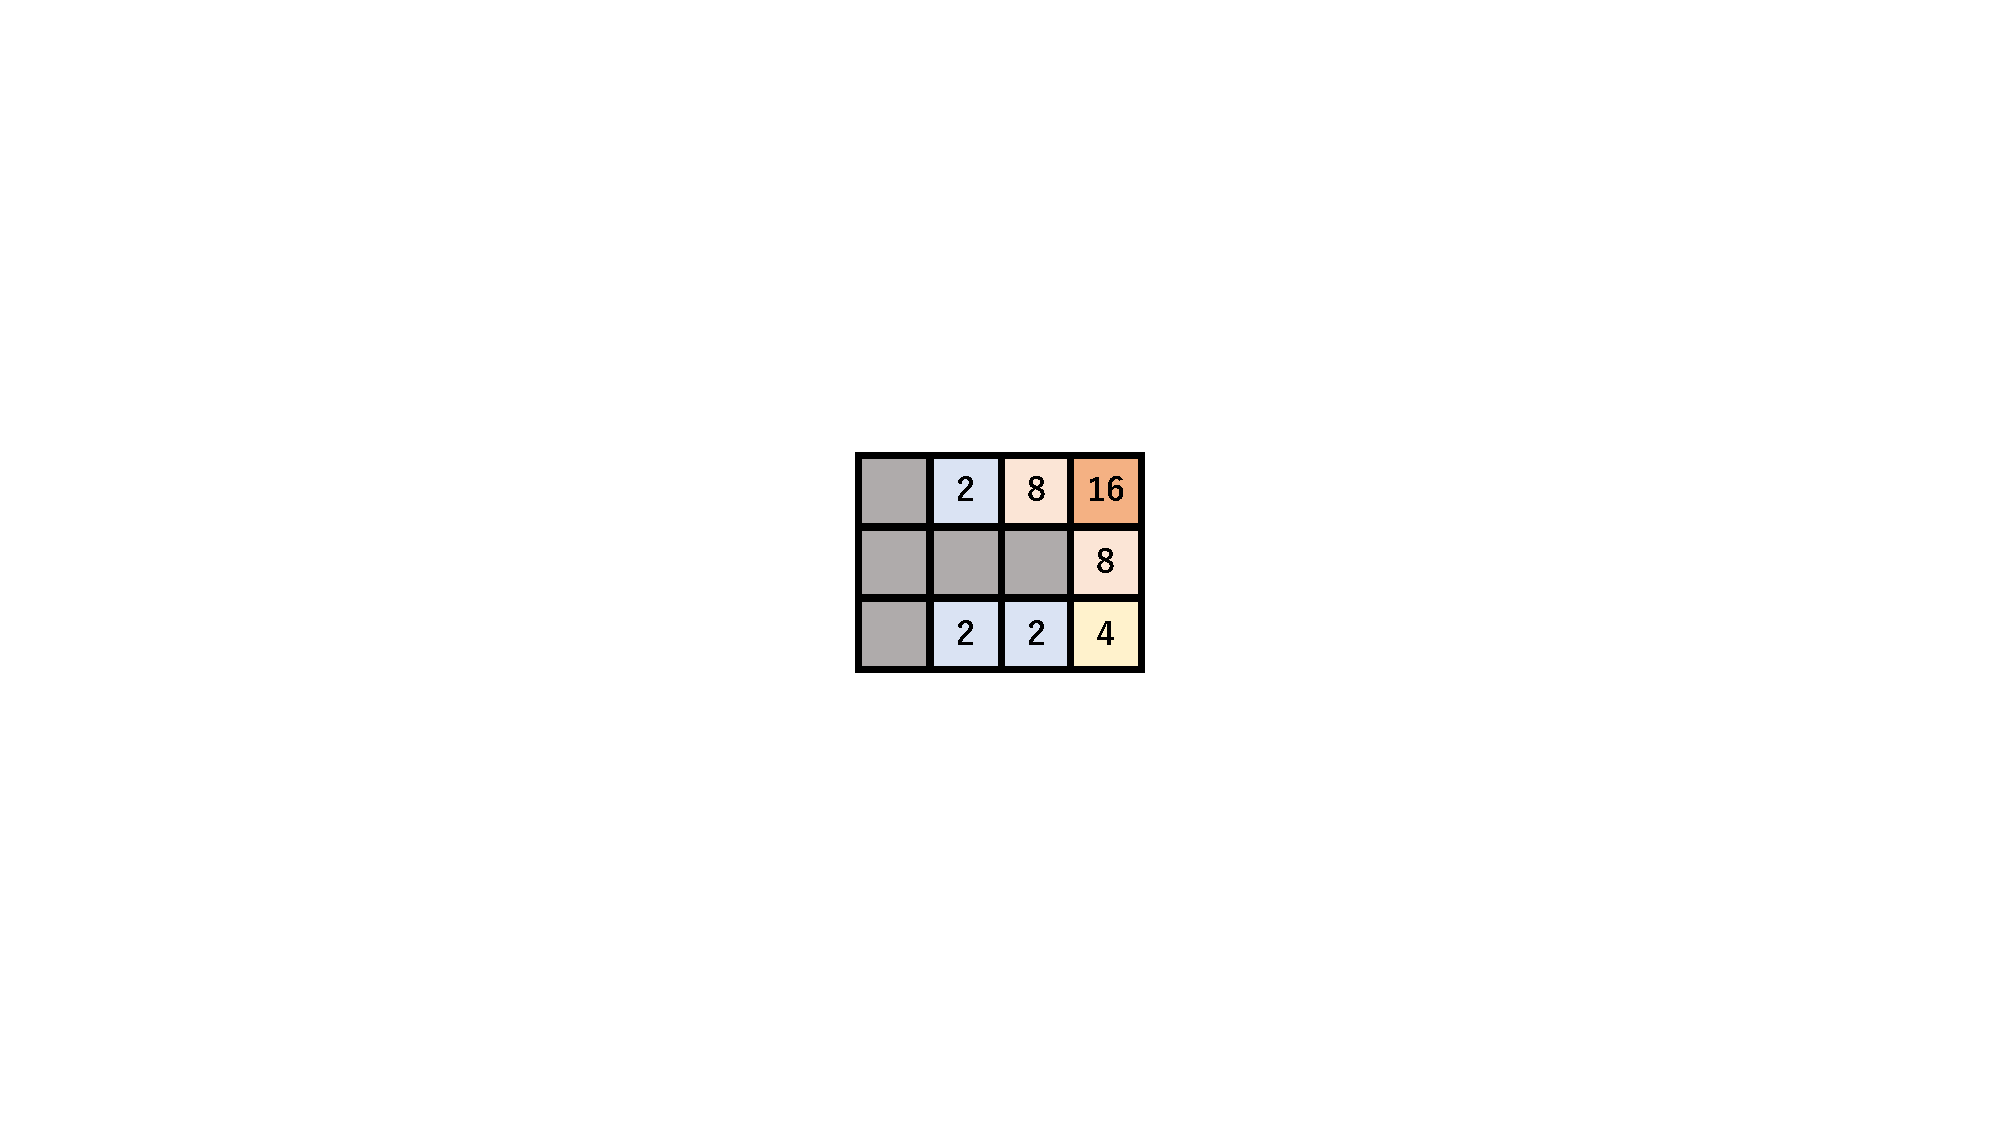
\includegraphics[width=\columnwidth]{figures/mid2048.pdf}
    \caption{$4\times3$盤面の2048}
    \label{fig:mid2048}
\end{subfigure}
\label{fig:minigames}
\end{figure}

\subsection{盤面サイズが小さな2048の完全解析}
\label{sec:mini2048}
基本的なルールは2048と同じで盤面サイズを$4\times4$から縮小したゲームを完全解析することを考える.
盤面サイズに関わらず, 以下の$2$つのステップを順番に行うことで完全解析を実行することができる.
\begin{enumerate}
    \item 初期状態から到達し得るすべての状態の列挙
    \item 列挙した状態の最適価値の計算
\end{enumerate}

\subsubsection{初期状態から到達し得るすべての状態の列挙}
\label{subsec:enumeration}
完全解析の第1ステップとしてゲームに現れうるすべての状態を列挙する.
これまでに発見した状態の集合$S$から状態を$1$つ取り出し, $s$から遷移可能な次の状態$s_{\text{next}} \in \mathcal{T}(s)$の内, 未発見の状態を$S$に追加する.
初期状態を$S$に入れて列挙を開始し, 新たに発見する状態がなくなるまで繰り返すことで, すべての状態を列挙することができる.

素朴な方法ではこれまでに発見した状態の集合$S$をメモリ上で管理することが考えられるが, 状態数が非常に大きな場合にはメモリの容量を超えてしまう.
そこで~\ref{sec:property}節で説明した時刻によって, ゲーム木を整理しこれを解決する.
時刻$t$の状態は時刻$t+2$か$t+4$の状態にしか遷移しないため, 時刻$t+2$と$t+4$の発見した状態の集合$S_{t+2}$と$S_{t+4}$をメモリ上で管理すれば十分である.
よって時刻が最小の$4$の状態から時刻$2$刻みで順番に列挙を行うことで, ディスクを効率的に活用することができる.
以上を踏まえた疑似コードをAlgorithm~\ref{alg:bfs}に示す.

\begin{algorithm}[tb]
\caption{すべての状態の列挙}
\label{alg:bfs}
\begin{algorithmic}[1]
\Function {enumerate}{}
    \State INITIALIZE($S_4, S_6, S_8$)
    \For {$t=4$ to $t_{\text{max}}$}
        \ForAll {$s_t \in S_t$} 
            \ForAll {$s_{t+2} \in \mathcal{T}(s_t)$}
                \If {$s_{t+2} \notin S_{t+2}$} 
                    \State $S_{t+2} = S_{t+2} \cup \{s_{t+2}\}$
                \EndIf
            \EndFor
            \ForAll {$s_{t+4} \in \mathcal{T}(s_t)$}
                \If {$s_{t+4} \notin S_{t+4}$} 
                    \State $S_{t+4} = S_{t+4} \cup \{s_{t+4}\}$
                \EndIf
            \EndFor
        \EndFor
    \EndFor
\EndFunction
\end{algorithmic}
\end{algorithm}

\subsubsection{後退解析による状態の最適価値の計算}
\label{subsec:calculation}
\ref{subsec:enumeration}節で列挙した状態の価値を, 式~\ref{eq:value}に従って後退解析を行い計算する.
状態列挙のときと同様に, 時刻に従って状態を管理することで効率的に後退解析を行える.
すなわち時刻$t$の状態の価値は, 時刻$t+2$と$t+4$の状態の価値が計算済みであれば必ず計算できる.
よって時刻が最大の状態から順番に走査することで, 無駄なくすべての状態の価値を計算できる.
疑似コードをAlgorithm~\ref{alg:calculation}に示す.
\begin{algorithm}[tb]
    \begin{algorithmic}[1]
    \Function {retrograde}{}
        \For {$t=t_{\text{max}}$ to $4$}
            \ForAll {$s_t \in S_t$} 
                \If {$s_t$ is gameover}
                    \State $v_*(s_t) = 0$
                \Else {}
                    \State $v_*(s_t) = \max_a \left(r(s_t,a) + \mathbb{E}_{s_\text{next} \in \mathcal{T}(s_t,a)} v_*(s_\text{next}) \right)$
                \EndIf
            \EndFor
        \EndFor
    \EndFunction
    \end{algorithmic}
    \caption{後退解析による価値計算}
    \label{alg:calculation}
\end{algorithm}

\subsection{実験結果}
本研究では$2\times2$盤面から$4\times3$盤面までの2048を完全解析することに成功した.
完全解析した結果を表~\ref{table: analysis_table}に示す.
\begin{table}[t]
    \centering
    \begin{tabular}{lrr}
        \hline \hline
        盤面サイズ & 状態数 & 初期状態の価値\\ \hline
        $2\times2=4$ & $110$ & $67.6$ \\
        $3\times2=6$ & $21,752$ & $480.9$ \\
        $4\times2=8$ & $4,980,767$ & $2,642.6$ \\
        $3\times3=9$ & $48,713,519$ & $5,468.4$ \\
        $4\times3=12$ & $1,152,817,492,752$ & $50,724.2$ \\
        \hline
    \end{tabular}
    \caption{盤面の大きさと解析結果に関する表}
    \label{table: analysis_table}
\end{table}
盤面サイズが大きくなるに従って指数関数的に状態数は大きくなることが分かる.
そのため$4\times4$盤面の2048は完全解析を行うには状態数が非常に大きいことが予想される.
一方で初期状態の最適価値は, 盤面サイズが$n$マス増える度に$2^n \sim 2^{n+1}$倍になっていることが見て取れる.
よって$4\times4$盤面の2048では初期状態の最適価値は, 少なく見積もっても$800,000$点程度はあるのではないかと推測される.

$3\times3$盤面と$4\times3$盤面の2048の各時刻における状態数のグラフを図~\ref{fig:state_afterstate}に示す.
多くのゲームでは進行に従って多様な盤面が存在するため状態数は大きくなり続ける.
一方で2048は盤面が数字タイルで埋まるとゲームオーバーになりやすく, その時刻の状態数は少なくなる.
大きな数字タイルを完成させると盤面上に空きマスが増え, ゲームは再び複雑性を増す.
実際, 図~\ref{fig:state_afterstate}からは$2^n$の前後の時刻で状態数が大きく増減していることが見て取れる.
よって2048はゲームの進行に従って, ゲームの複雑性が増減するという特徴を持つといえる.
\begin{figure} 
\vspace{0.2cm}
\begin{subfigure}[T]{0.4\columnwidth}
    \centering
    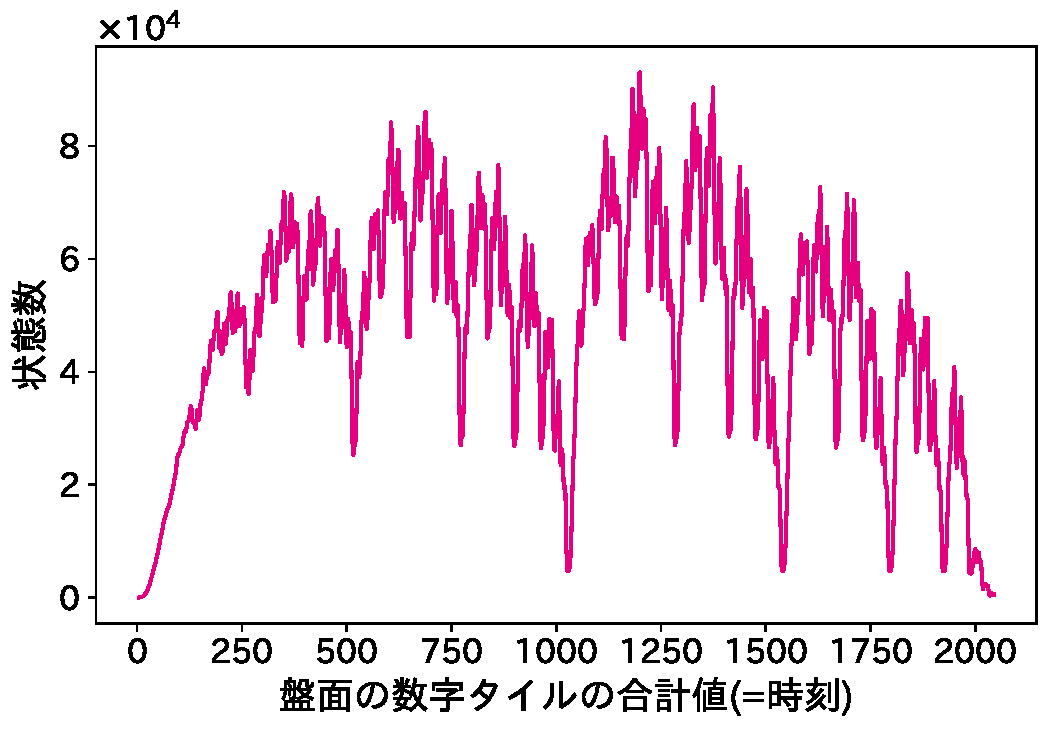
\includegraphics[width=\columnwidth]{figures/graph_mini.pdf}
    \caption{$3\times3$盤面の2048の時刻と状態数}
    \label{fig:graph_mini}
\end{subfigure}
\hspace{1cm}
\begin{subfigure}[T]{0.4\columnwidth}
    \centering
    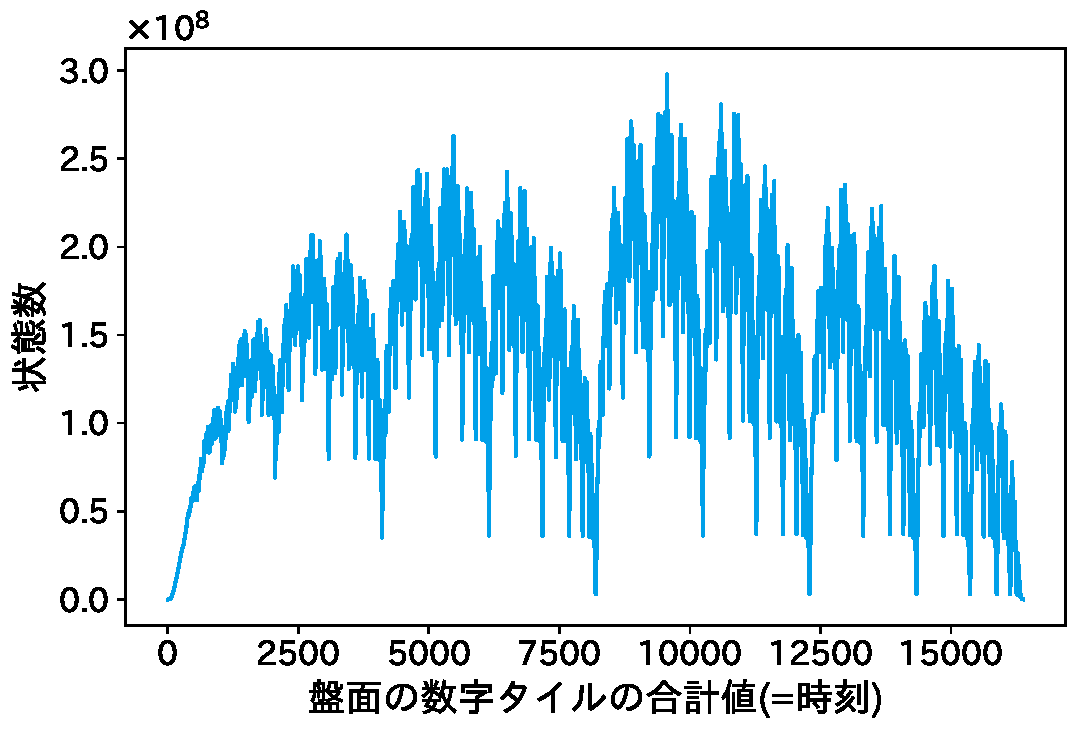
\includegraphics[width=\columnwidth]{figures/graph_mid.pdf}
    \caption{$4\times3$盤面の2048の時刻と状態数}
    \label{fig:graph_mid}
\end{subfigure}
\label{fig:time_state_num}
\end{figure}
参考として, $2\times2$盤面の2048のゲーム木全体を図~\ref{fig:game_tree}に示す.
ゲーム木が拡大と縮小を繰り返す様子が見て取れる.
\begin{figure}[t]
    \centering
    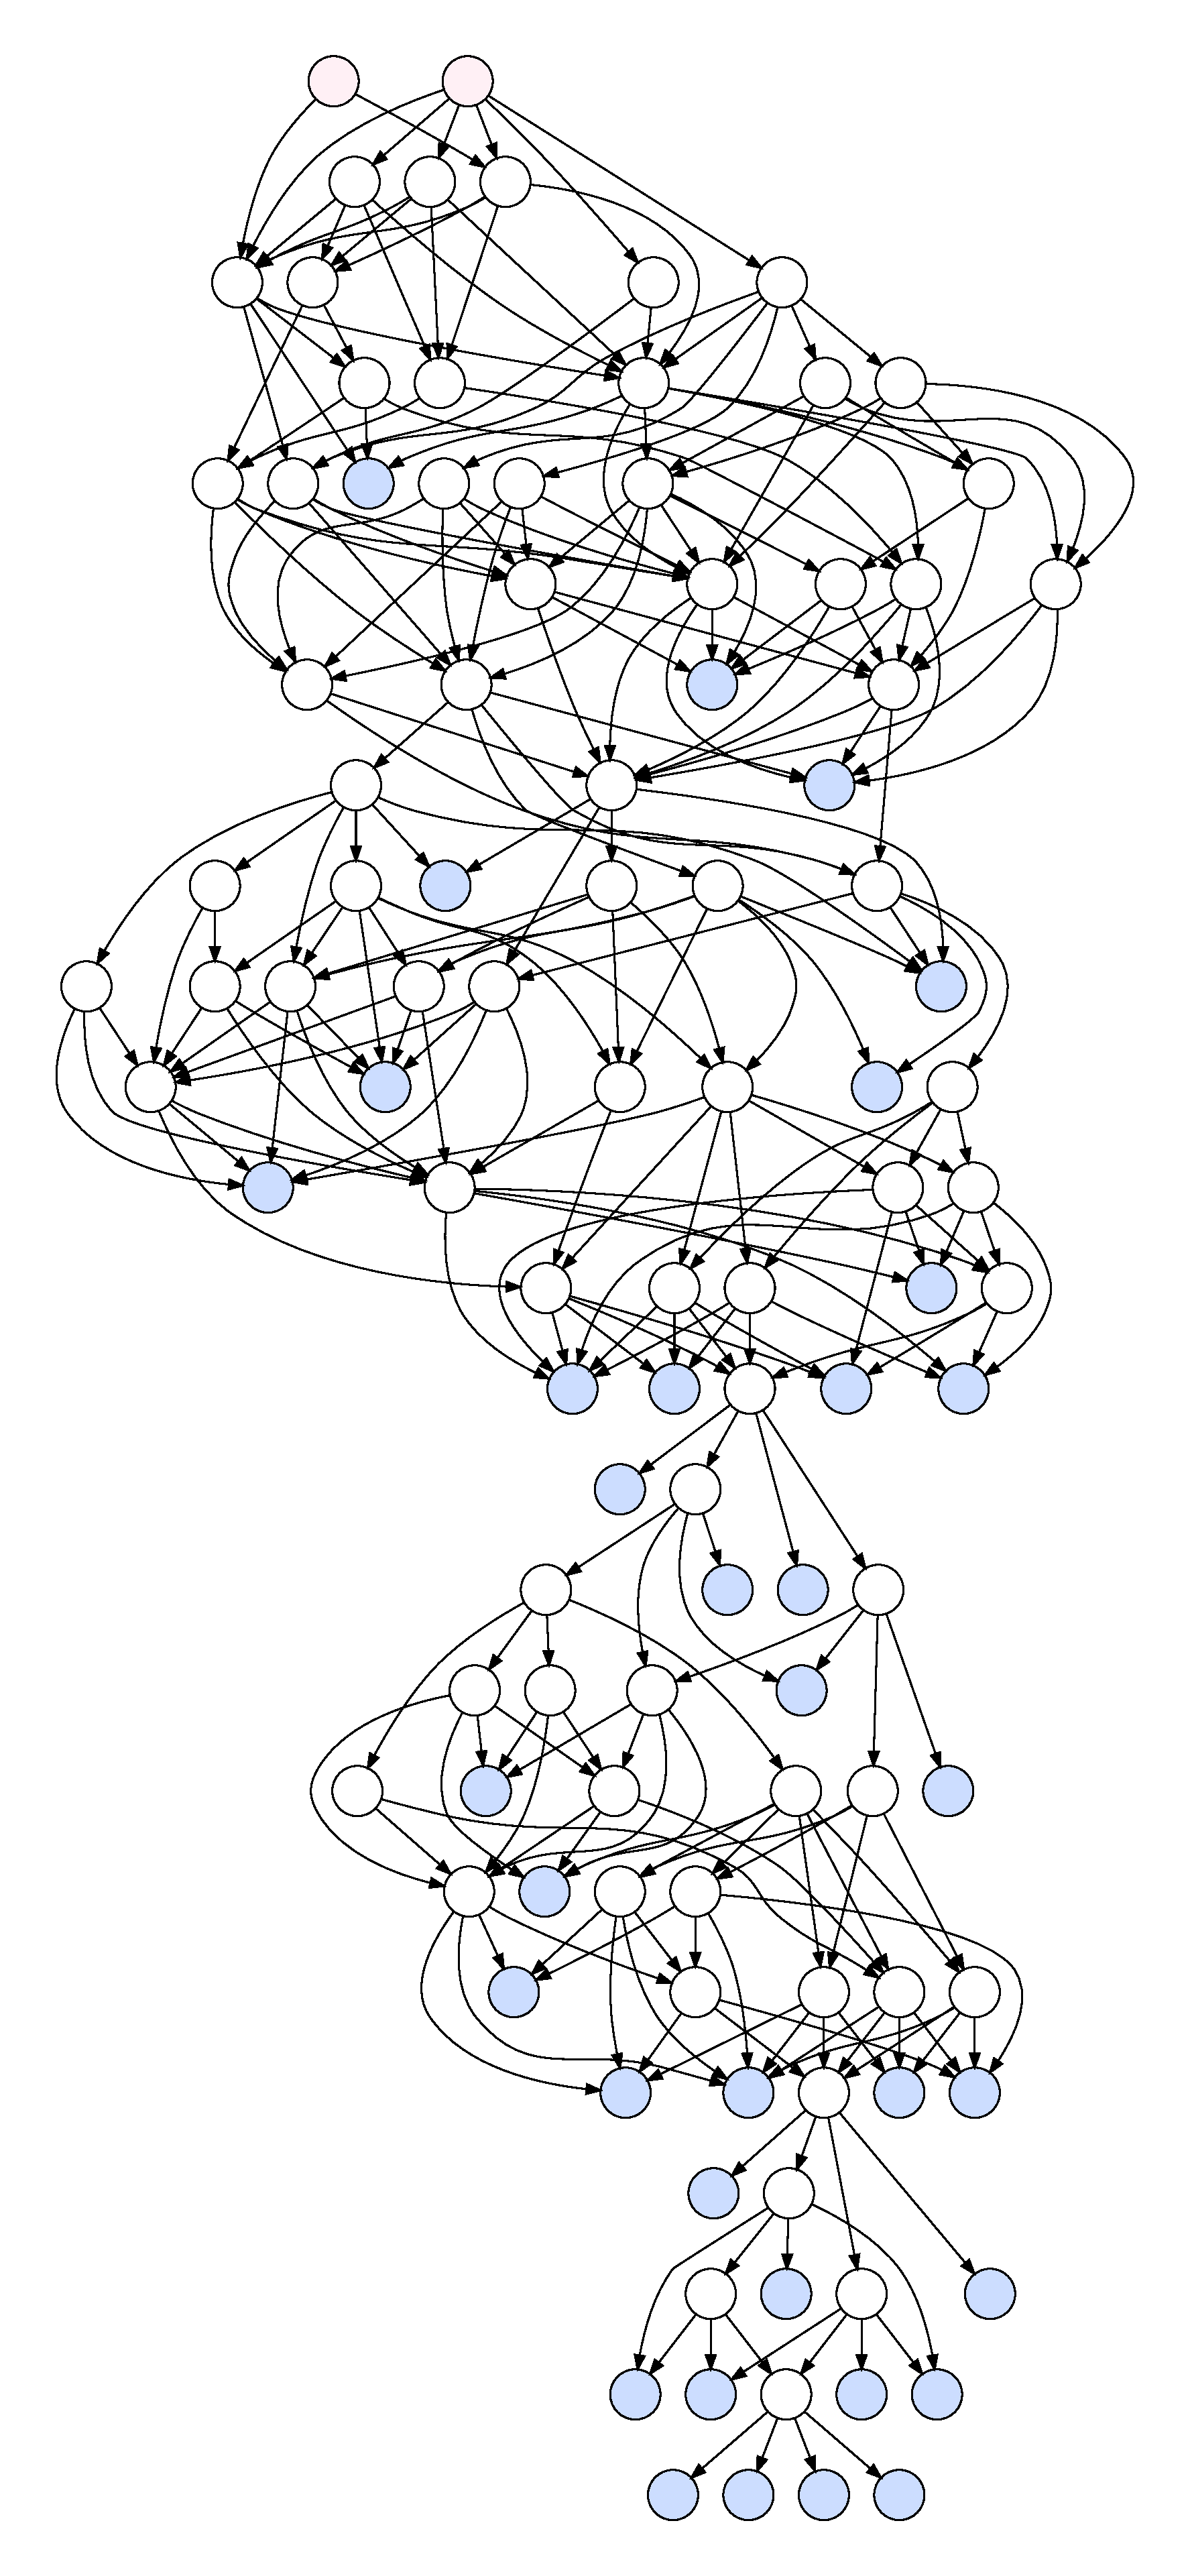
\includegraphics[width=0.7\linewidth{}]{figures/tree.pdf}
    \caption{$2\times2$盤面の2048のゲーム木~(赤色のノードは初期状態, 青色のノードは終了状態)}
    \label{fig:game_tree}
\end{figure}